%%%%%%%%%%%%%%%%%%%%%%%%%%%%%%%%%%%%%%%%%
% HW Template
% LaTeX Template
% Version 1.0 (19/10/18)
% Modified by
% Erdem TUNA
% Halil TEMURTAŞ 
% Enes TAŞTAN 
%%%%%%%%%%%%%%%%%%%%%%%%%%%%%%%%%%%%%%%%%
%
%----------------------------------------------------------------------------------------
%	PACKAGES AND OTHER DOCUMENT CONFIGURATIONS
%----------------------------------------------------------------------------------------
\documentclass[a4paper,12pt]{article}
%-----packages------
\usepackage[a4paper, total={6.2in, 8.5in}]{geometry}
\usepackage[english]{babel}
\usepackage[utf8x]{inputenc}
\usepackage{amsmath}
\usepackage{graphicx}
\usepackage[colorinlistoftodos]{todonotes}
\usepackage{gensymb} % this could be problem
\usepackage{float}
\usepackage{fancyref}
\usepackage{subcaption}
\usepackage[toc,page]{appendix} %appendix package
\usepackage{xcolor}
\usepackage{listings}
\usepackage{xspace}
\usepackage{amssymb}
\usepackage{nicefrac}
\usepackage{gensymb}
\usepackage{fancyhdr}
\usepackage{blindtext}  % for dummy text, use \blindtext or \BlindText
\usepackage{lipsum}    % for dummy text, use \lipsum[3-56]
\usepackage[final]{pdfpages}  % pdf include
\usepackage{array} %allows more options in tables
\usepackage{pgfplots,pgf,tikz} %coding plots in latex
\usepackage{capt-of} % allows caption outside the figure environment
\usepackage[export]{adjustbox} %more options for adjusting the images
\usepackage{multicol,multirow,slashbox} % allows tables like table1
%\usepackage[hyperfootnotes=false]{hyperref} % clickable references
\usepackage{epstopdf} % useful when matlab is involved
%\usepackage{placeins} % prevents the text after figure to go above figure with \FloatBarrier 
%\usepackage{listingsutf8,mcode} %import .m or any other code file mcode is for matlab highlighting
\usepackage{enumitem}
\usepackage{hyperref}

%-----end of packages

%-----specifications-----
\definecolor{mGreen}{rgb}{0,0.6,0} % for python
\definecolor{mGray}{rgb}{0.5,0.5,0.5}
\definecolor{mPurple}{rgb}{0.58,0,0.82}
\definecolor{mygreen}{RGB}{28,172,0} % color values Red, Green, Blue for matlab
\definecolor{mylilas}{RGB}{170,55,241}

\setcounter{secnumdepth}{5} % how many sectioning levels to assign numbers to
\setcounter{tocdepth}{5}    % how many sectioning levels to show in ToC

\lstdefinestyle{CStyle}{
	commentstyle=\color{mGreen},
	keywordstyle=\color{magenta},
	numberstyle=\tiny\color{mGray},
	stringstyle=\color{mPurple},
	basicstyle=\footnotesize,
	breakatwhitespace=false,         
	breaklines=true,
	frame=single,
	rulecolor=\color{black!40},                 
	captionpos=b,                    
	keepspaces=true,                 
	numbers=left,                    
	numbersep=5pt,                  
	showspaces=false,                
	showstringspaces=false,
	showtabs=false,                  
	tabsize=2,
	language=C
}

\lstset{language=Matlab,%
	%basicstyle=\color{red},
	breaklines=true,%
	frame=single,
	rulecolor=\color{black!40},
	morekeywords={matlab2tikz},
	keywordstyle=\color{blue},%
	morekeywords=[2]{1}, keywordstyle=[2]{\color{black}},
	identifierstyle=\color{black},%
	stringstyle=\color{mylilas},
	commentstyle=\color{mygreen},%
	showstringspaces=false,%without this there will be a symbol in the places where there is a space
	numbers=left,%
	numberstyle={\tiny \color{black}},% size of the numbers
	numbersep=9pt, % this defines how far the numbers are from the text
	emph=[1]{for,end,break},emphstyle=[1]\color{red}, %some words to emphasise
	%emph=[2]{word1,word2}, emphstyle=[2]{style},    
}


\tikzset{
	desicion/.style={
		diamond,
		draw,
		text width=4em,
		text badly centered,
		inner sep=0pt
	},
	block/.style={
		rectangle,
		draw,
		text width=10em,
		text centered,
		rounded corners
	},
	cloud/.style={
		draw,
		ellipse,
		minimum height=2em
	},
	descr/.style={
		fill=white,
		inner sep=2.5pt
	},
	connector/.style={
		-latex,
		font=\scriptsize
	},
	rectangle connector/.style={
		connector,
		to path={(\tikztostart) -- ++(#1,0pt) \tikztonodes |- (\tikztotarget) },
		pos=0.5
	},
	rectangle connector/.default=-2cm,
	straight connector/.style={
		connector,
		to path=--(\tikztotarget) \tikztonodes
	}
}

\tikzset{
	desicion/.style={
		diamond,
		draw,
		text width=4em,
		text badly centered,
		inner sep=0pt
	},
	block/.style={
		rectangle,
		draw,
		text width=10em,
		text centered,
		rounded corners
	},
	cloud/.style={
		draw,
		ellipse,
		minimum height=2em
	},
	descr/.style={
		fill=white,
		inner sep=2.5pt
	},
	connector/.style={
		-latex,
		font=\scriptsize
	},
	rectangle connector/.style={
		connector,
		to path={(\tikztostart) -- ++(#1,0pt) \tikztonodes |- (\tikztotarget) },
		pos=0.5
	},
	rectangle connector/.default=-2cm,
	straight connector/.style={
		connector,
		to path=--(\tikztotarget) \tikztonodes
	}
}
%-----end of specifications-----


%----commands----
\newcommand\nd{\textsuperscript{nd}\xspace}
\newcommand\rd{\textsuperscript{rd}\xspace}
\newcommand\nth{\textsuperscript{th}\xspace} %\th is taken already
\newcommand{\specialcell}[2][c]{ \begin{tabular}[#1]{@{}c@{}}#2\end{tabular}} % for too long table lines

\newcommand{\blankpage}{
	\- \\[9cm]	
	{ \centering \textit{This page intentionally left blank.} \par }
	\- \\[9cm]
}% For Blank Page

\makeatletter
\renewcommand\paragraph{\@startsection{paragraph}{4}{\z@}%
	{-2.5ex\@plus -1ex \@minus -.25ex}%
	{1.25ex \@plus .25ex}%
	{\normalfont\normalsize\bfseries}}
\makeatother
%-----end of commands-----

\pagestyle{fancy}
\fancyhead[LO,LE]{Halil TEMURTAŞ / 2094522 }
\fancyhead[RO,RE]{December 3, 2018}
\fancyfoot[RO,RE]{
\includegraphics[width=2.7cm]{images/eelogo}}

\begin{document}
\begin{center}
	\textbf{\large EE407 Process Control \\[0.2cm] Experiment 5} \\
\end{center}


	\begin{enumerate}
		\item Reverting back to actual temperature, 
			
			$$ T(x,t)=T_e+(M-T_e)erfc(\frac{x}{2\sqrt{\alpha t}})\ for\ 𝑥>0\ and\ 𝑡>0$$		
			
			For our case;
			
			$$ T(L,t)=T_e+(M-T_e)erfc(\frac{L}{2\sqrt{\alpha t}}) $$
			
			with given constants and $T_e=0$ ,for convenience, and $M=1$ for unit step input;
			
			The response can be seen at \textit{Figure~\ref{fig:pre1}}. Source code for this part can be examined at \textbf{Appendix A}.
		
			\begin{figure}[H]
				\center
				\setlength{\unitlength}{\textwidth} 
				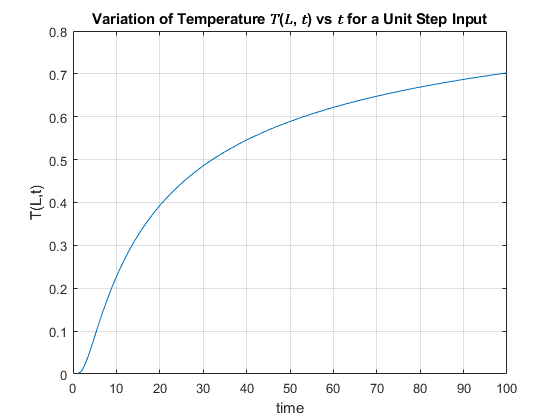
\includegraphics[width=0.8\unitlength]{images/pre1}
				\caption{\label{fig:pre1} Variations of Temperature T(L,t) vs time }
			\end{figure}
	
			
		\item In general,
		
			$$ \frac{1}{\alpha}\frac{dT_r(t)}{dt}=\frac{T_{r-1}(t)-2T_r(t)+T_{r+1}(t)}{{(\Delta x)}^2}\ for r=1,2, .... n$$
			
			$T_{n+1}$ can be assumed to be equal to $T_n$ for $n$ equations to solve for unknowns.
		
		
		\begin{itemize}
			\item for n=1
				$$ \frac{1}{\alpha}\frac{dT_1(t)}{dt}=\frac{T_0(t)-2T_1(t)+T_2(t)}{{(\Delta x)}^2}	$$		
				where $T_o$ is the input and $T_1=T_2$ assumption can be made.
				
				Taking Laplace transforms of both sides, it can be found that;
				
				$$ \left( \frac{{(\Delta x)}^2}{\alpha} s+1\right) T_1(s)=T_0(s)$$	
				
				$$ \frac{T_1(s)}{T_0(s)}=\cfrac{1}{\cfrac{{(\Delta x)}^2}{\alpha} s+1}$$
				
				it can be seen that the time constant of this equation is 
				
				$$ \tau_1=\frac{{(\Delta x)}^2}{\alpha}= 29.2002\ seconds$$
				
				where $\Delta x=L=5\ cm$.
				
				Let us now find the circuit equivalent of this approximation. The circuit at at \textit{Figure~\ref{fig:pre2a}} seems a good fit. Let us now analyse this circuit and find its time constant. It is desired that the time constant of this circuit should at lest $10^{-5}$ times of the approximation model.
				
				\begin{figure}[H]
					\center
					\setlength{\unitlength}{\textwidth} 
					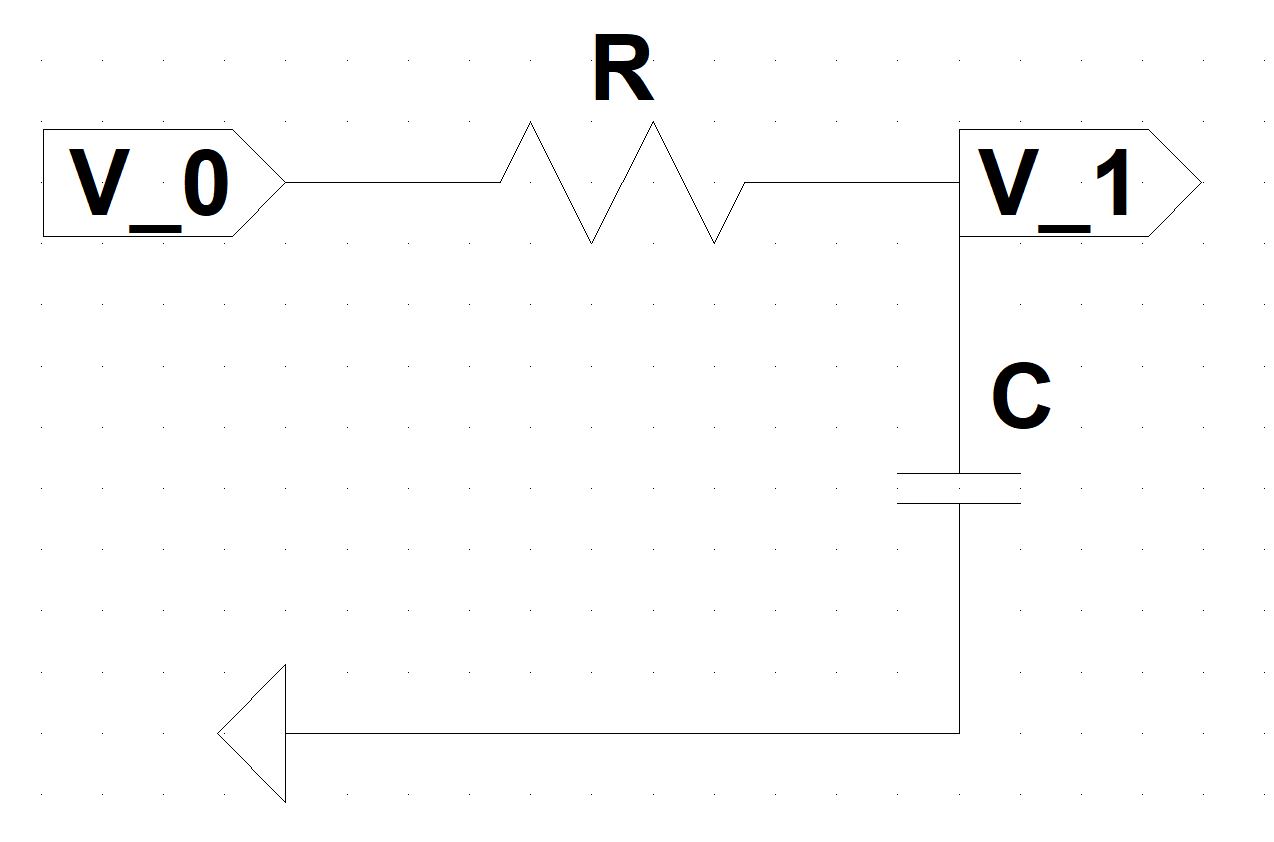
\includegraphics[width=0.6\unitlength]{images/pre2a}
					\caption{\label{fig:pre2a} Circuit Equivalent of Lumped Approximation Model for n=1}
				\end{figure}
				
				$$ \frac{V_1(s)}{V_0(s)}=\frac{1}{1+(RC)s}$$
				
				$$ \tau_c=RC=10^{-5}\tau_1=2.92\ 10^{-4}$$
				
				Assuming $C=1\ \mu F$
				
				$R$ value can be found to be as $292.002\ \Omega$
				
			\item for n=2;
				$$ \frac{1}{\alpha}\frac{dT_1(t)}{dt}=\frac{T_0(t)-2T_1(t)+T_2(t)}{{(\Delta x)}^2}	$$		
				$$ \frac{1}{\alpha}\frac{dT_2(t)}{dt}=\frac{T_1(t)-2T_2(t)+T_3(t)}{{(\Delta x)}^2}	$$		
				where $T_o$ is the input and $T_2=T_3$ assumption can be made.
				
				Taking Laplace transform of both sides
				
				Assume from now on $A=\frac{{(\Delta x)}^2}{\alpha}$
				
				$$ (As+2)T_1(s)=T_0(s)+T_2(s)$$
				
				$$ (As+1)T_2(s)=T_1(s)$$
				
				$$ [(As+2)(As+1)-1]T_2(s)=T_0(s) $$
				
				$$ \frac{T_2(s)}{T_0(s)}=\frac{1}{A^2s^2+3As+1}=\frac{1}{\tau_2^2s^2+ 2 \xi \tau_2 +1} $$
	
				with $\Delta x=L/2=2.5 cm$
								
				$$ \tau_2=A= \frac{{(\Delta x)}^2}{\alpha} = 7.3001\ secs $$
				
				Desired time constant for circuit equivalent then $\tau_{c2}=10^{-5}\ \tau_2=7.3\ 10^{-5}\ secs$ 
				
				\begin{figure}[H]
					\center
					\setlength{\unitlength}{\textwidth} 
					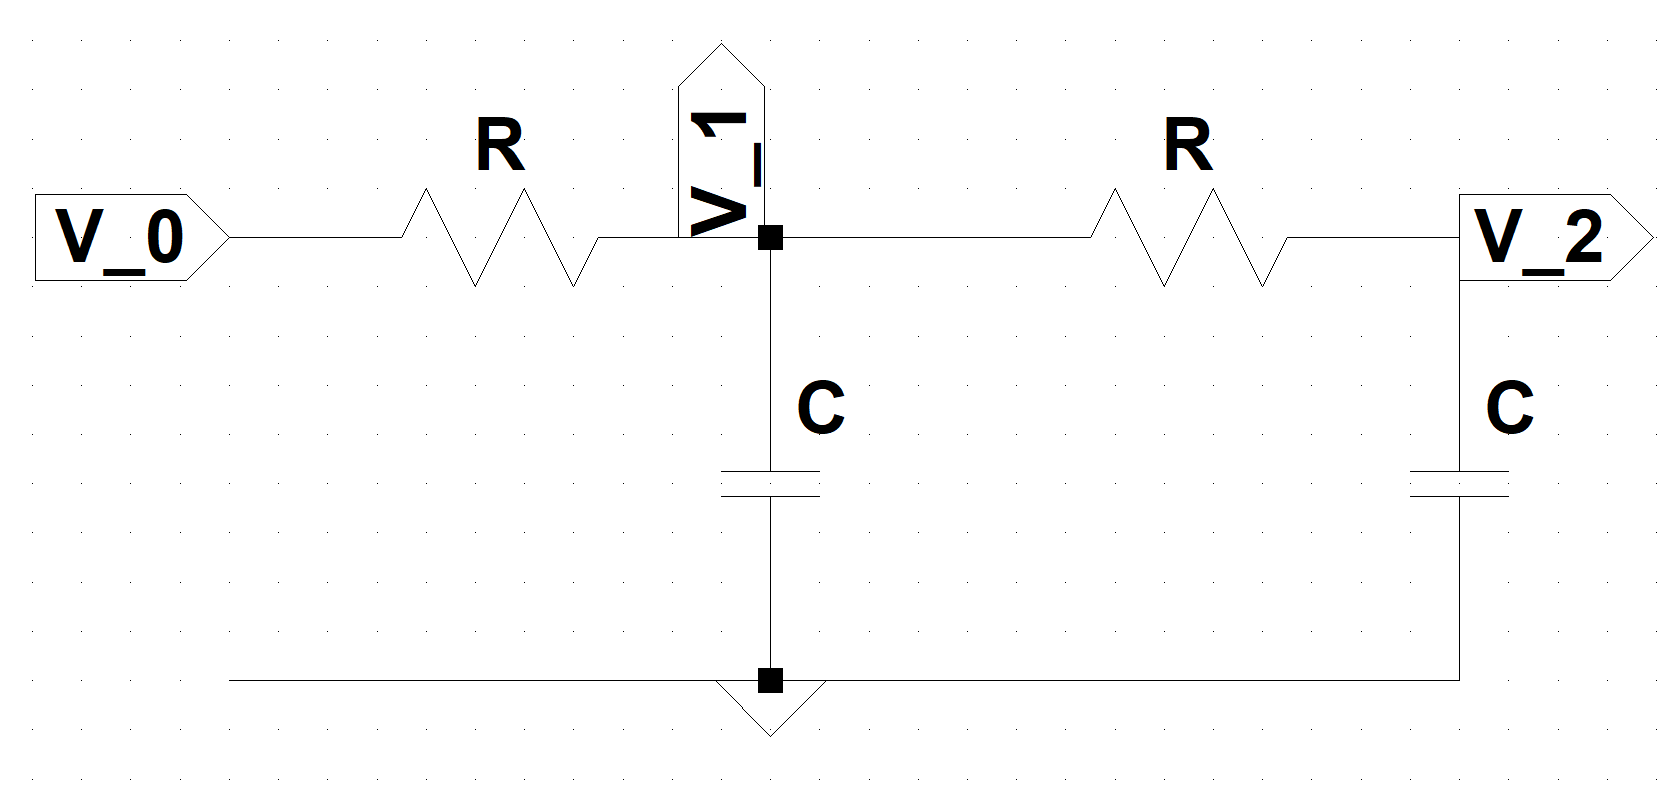
\includegraphics[width=0.6\unitlength]{images/pre2b}
					\caption{\label{fig:pre2b} Circuit Equivalent of Lumped Approximation Model for n=2}
				\end{figure}
				

				The transfer equation for the circuit at \textit{Figure~\ref{fig:pre2b}} can be found as
									
				$$ \frac{V_2(s)}{V_1(s)}=\frac{1}{{(RC)}^2s^2+3(RC)s+1}==\frac{1}{\tau_{c2}^2s^2+ 2 \xi \tau_{c2} +1}				$$
				
				$$ \tau_{c2}=RC=7.3\ 10^{-5}\ secs$$
				
				Assuming $C=1\ \mu F$
				
				$R$ value can be found to be as $73.0005\ \Omega$
				
				\item for n, the circuit model at \textit{Figure~\ref{fig:pre2c}} can be used
				
					\begin{figure}[H]
						\center
						\setlength{\unitlength}{\textwidth} 
						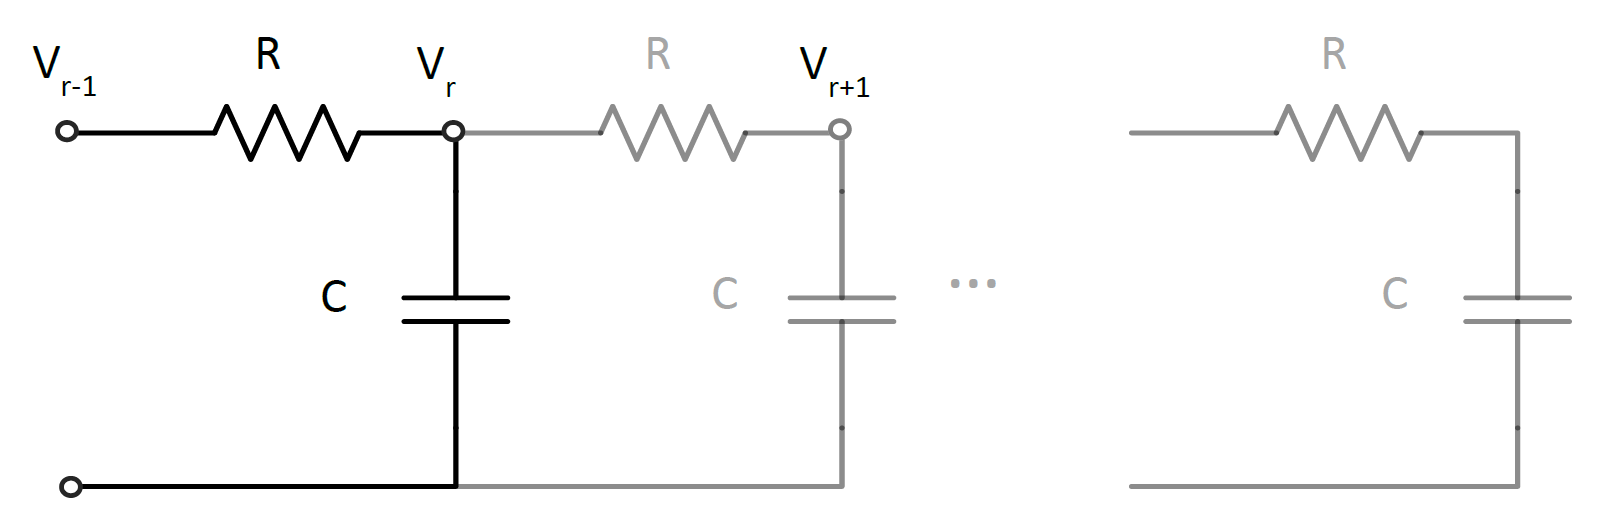
\includegraphics[width=0.9\unitlength]{images/pre2c}
						\caption{\label{fig:pre2c} Simulation of the lumped approximate model}
					\end{figure}
				
					The pattern can be observed from the first two equations that found earlier for $n=1,2$
				
				
					$$ \Delta x = \frac{L}{n} $$
				
					$$ \alpha = \frac{\lambda}{\rho c} $$
				
					$$ \tau_n=A= \frac{{(\Delta x)}^2}{\alpha}  $$
				
				
					$$ \tau_{cn}=RC=\tau_n 10^{-5} $$
				
				\item for n=3
							
					$$ \Delta x = \frac{L}{3} $$
				
					$$ \tau_3=A= 3.2445\ secs $$
				
					$$ \tau_{c3}=RC=\tau_3 10^{-5}=3.2445\ 10^{-5}\ secs  $$
					
					Assuming $C=1\ \mu F$
				
					$R$ value can be found to be as $ 32.4447\ \Omega$
					
				\item for n=5
							
					$$ \Delta x = \frac{L}{5} $$
				
					$$ \tau_5=A= 1.1680\ secs $$
				
					$$ \tau_{c5}=RC=\tau_5 10^{-5}=1.1680\ 10^{-5}\ secs  $$
					
					Assuming $C=1\ \mu F$
				
					$R$ value can be found to be as $ 11.6801\ \Omega$
				
			
		\end{itemize}
	
	

	
		\item The responses can be examined below
		
			
					\begin{figure}[H]
						\center
						\setlength{\unitlength}{\textwidth} 
						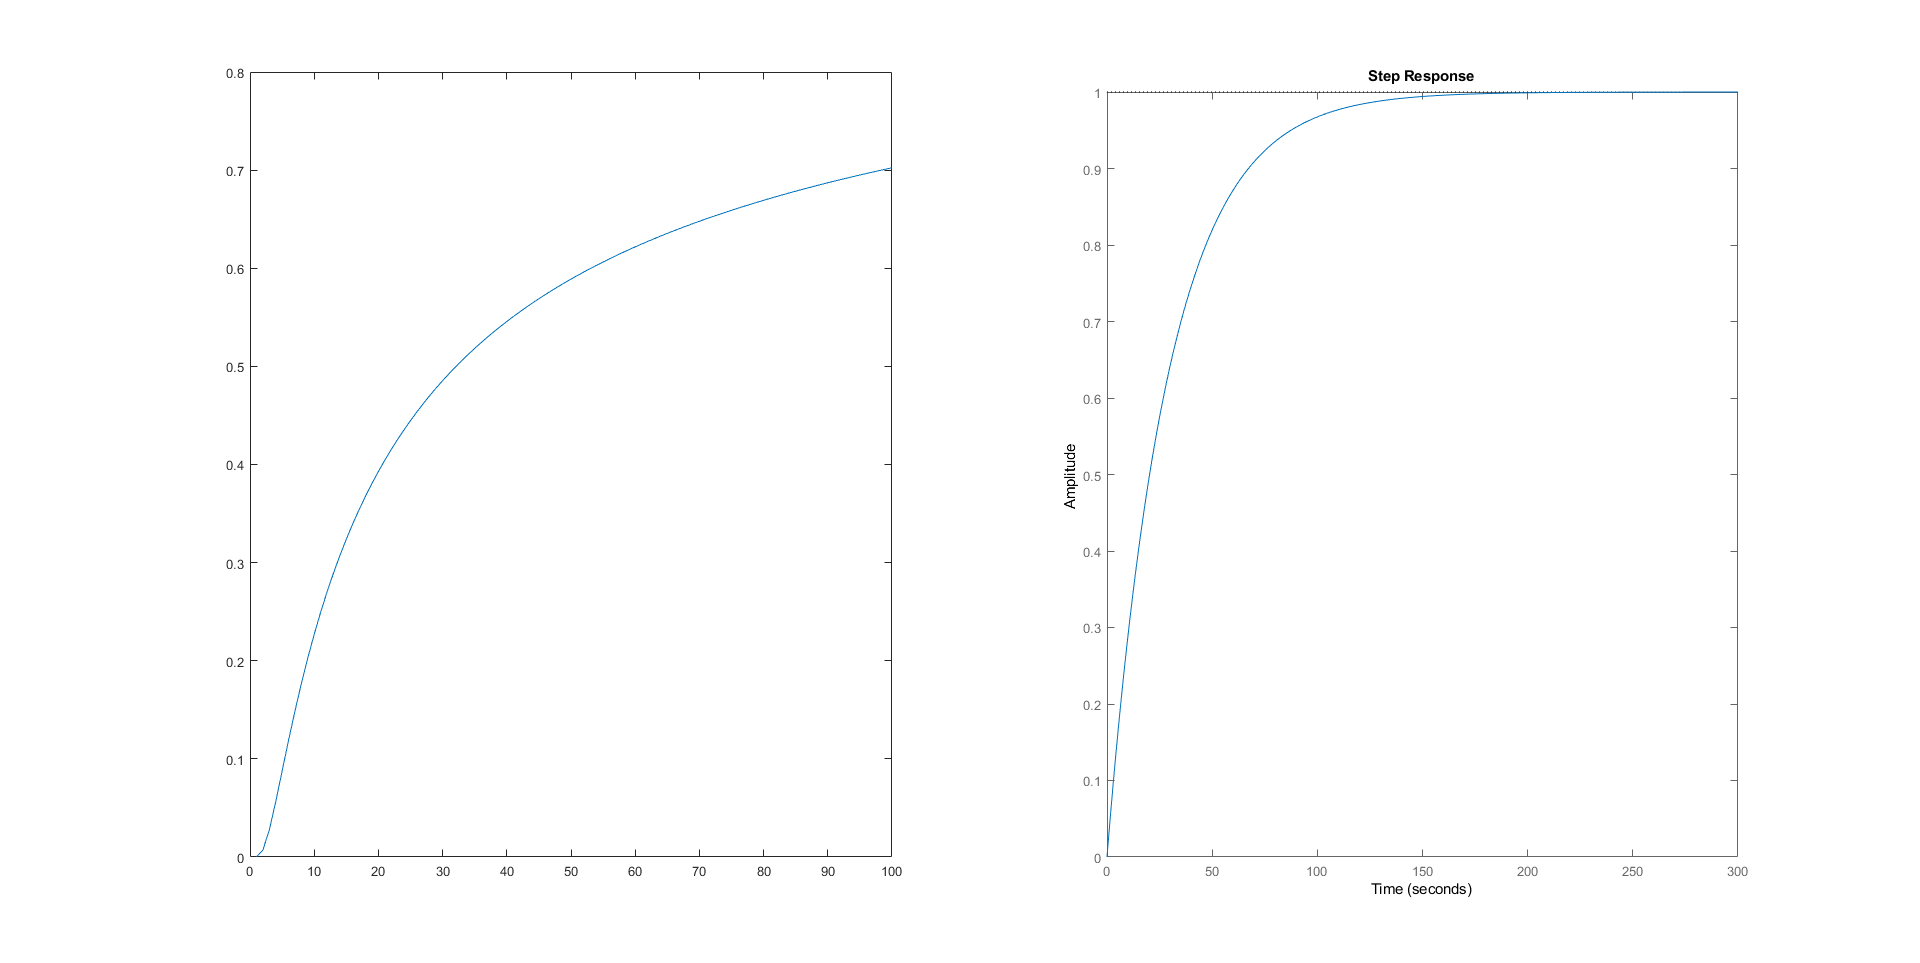
\includegraphics[width=0.9\unitlength]{images/3a}
						\caption{\label{fig:pre2c} Step response of System and steps response pf its Lumped Parameter approximation for n=1}
					\end{figure}
					
					
					\begin{figure}[H]
						\center
						\setlength{\unitlength}{\textwidth} 
						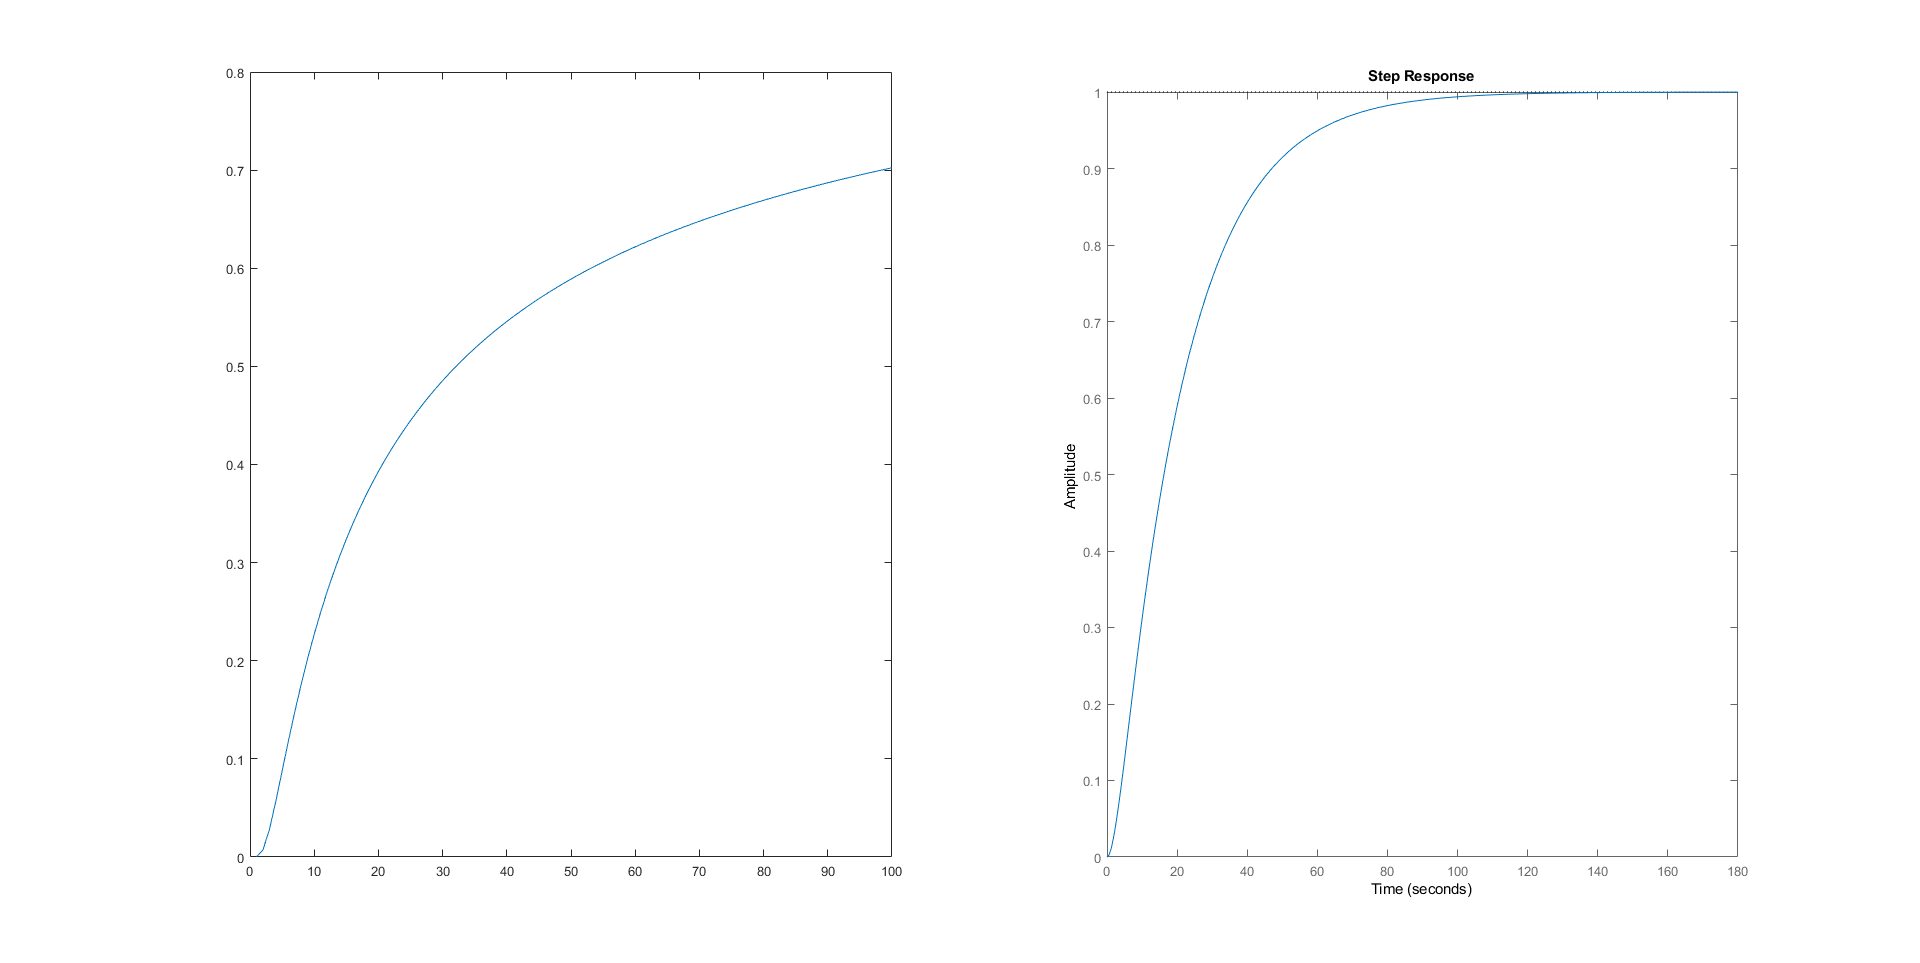
\includegraphics[width=0.9\unitlength]{images/3b}
						\caption{\label{fig:pre2c}  Step response of System and steps response pf its Lumped Parameter approximation for n=2}
					\end{figure}
					
					
					\begin{figure}[H]
						\center
						\setlength{\unitlength}{\textwidth} 
						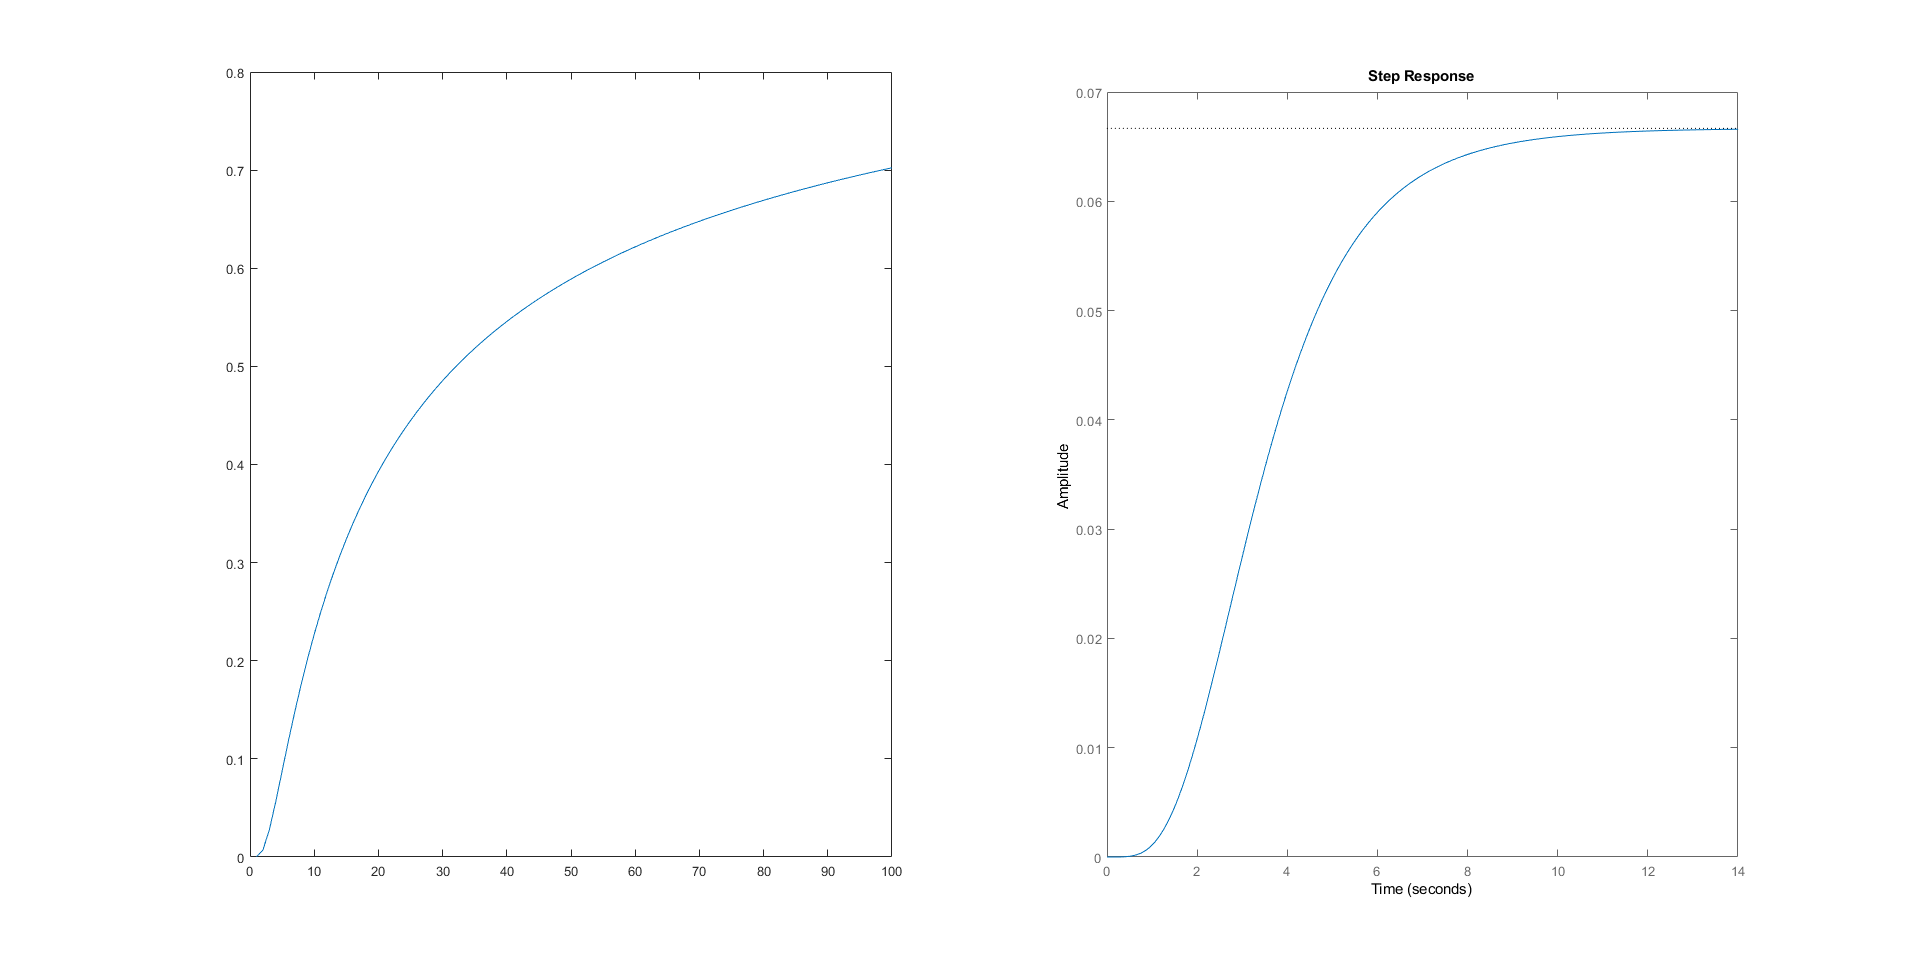
\includegraphics[width=0.9\unitlength]{images/3c}
						\caption{\label{fig:pre2c}  Step response of System and steps response pf its Lumped Parameter approximation for n=3}
					\end{figure}
					
					
					\begin{figure}[H]
						\center
						\setlength{\unitlength}{\textwidth} 
						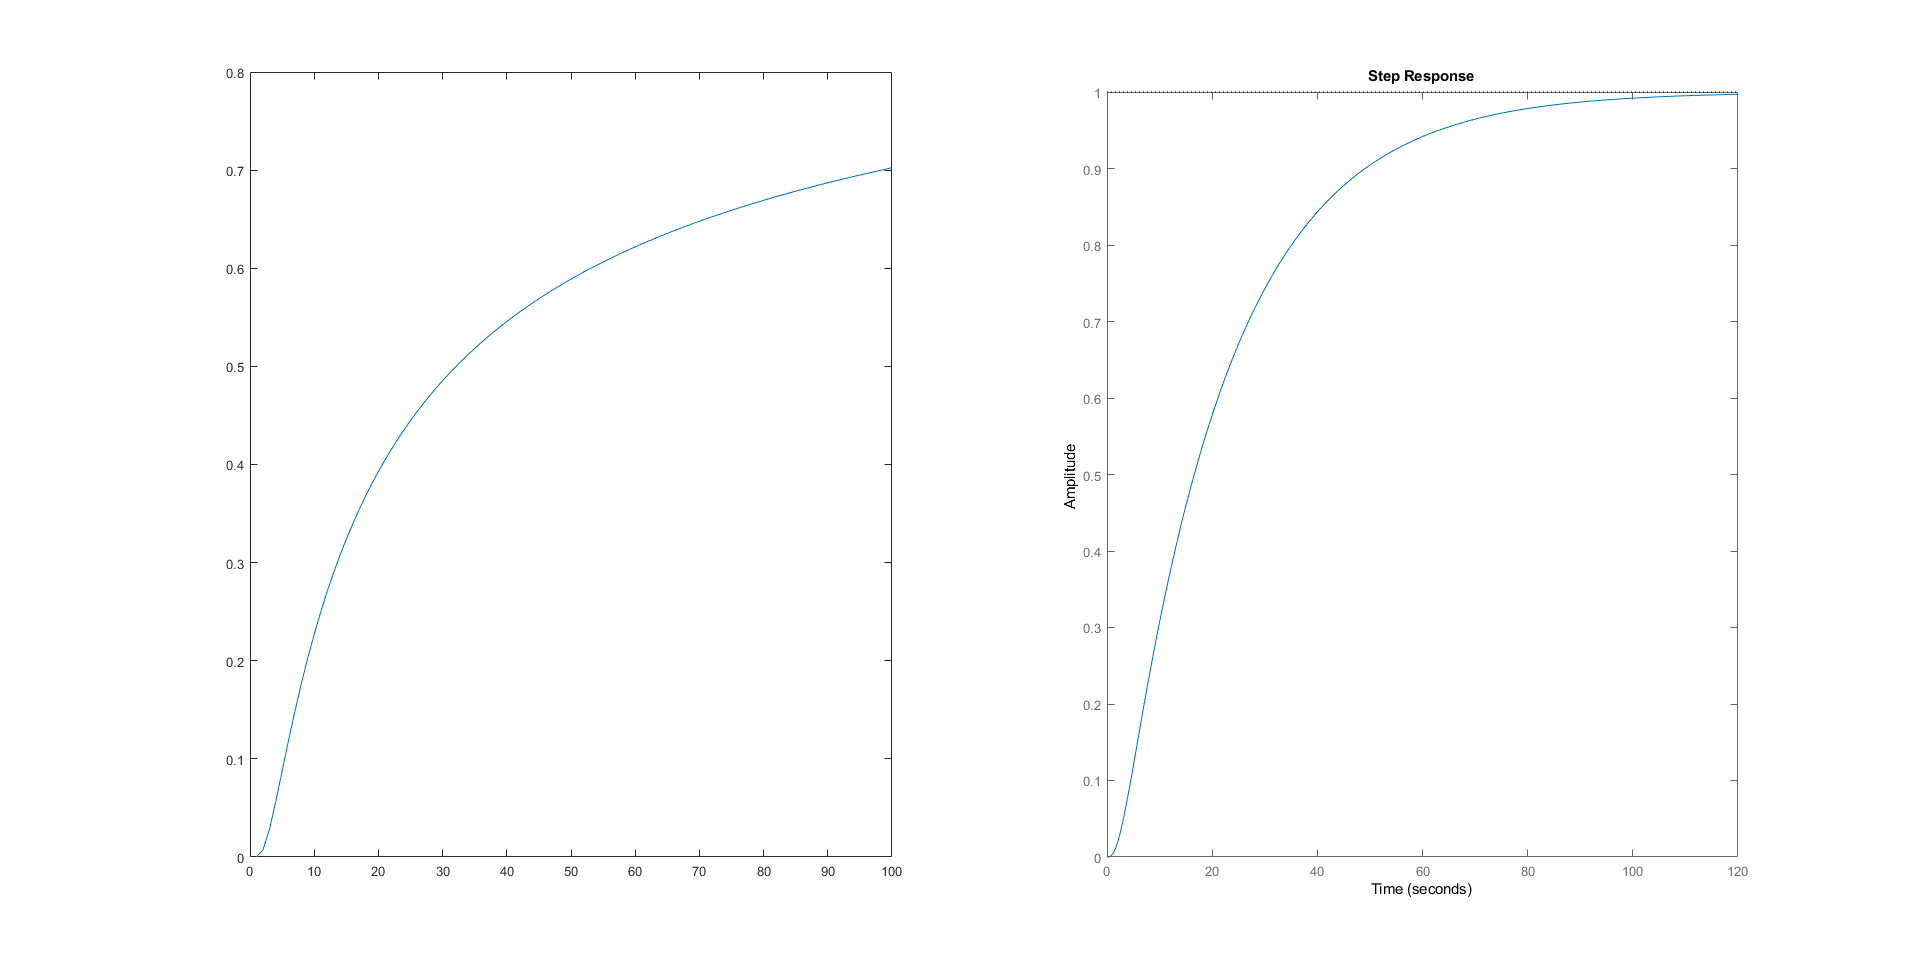
\includegraphics[width=0.9\unitlength]{images/3d}
						\caption{\label{fig:pre2c}  Step response of System and steps response pf its Lumped Parameter approximation for n=4}
					\end{figure}
			
		\end{enumerate}
		
		

	
\begin{appendices}
\section{Source Code for Matlab Part}\label{appendix}
	%%	\lstinputlisting[language=Matlab,firstline=33, lastline=34]{q13.m} \-\\[1cm]		
\lstinputlisting[language=Matlab]{Exp4.m} 
\end{appendices}

\end{document}

\end{document}

%----samples------
%\begin{itemize}
%\item Item
%\item Item
%\end{itemize}

%\begin{figure}[H]
%\center
%\setlength{\unitlength}{\textwidth} 
%\includegraphics[width=0.7\unitlength]{images/logo1}
%\caption{\label{fig:logo}Logo }
%\end{figure}

%\begin{figure}[H]
%	\setlength{\unitlength}{\textwidth} 
%	\centering
%	\begin{subfigure}{.5\textwidth}
%  		\centering
%  		\includegraphics[width=0.48\unitlength]{images/logo1}
%  		\caption{\label{fig:logo1}Logo1 }
%	\end{subfigure}%
%	\begin{subfigure}{.5\textwidth}
%  		\centering
%		\includegraphics[width=0.48\unitlength]{images/logo2}
%  		\caption{\label{fig:logo2}Logo2}
%	\end{subfigure}
%\caption{\label{fig:calisandegree} Small Logos   }
%\end{figure}
	
%\begin{table}[H]
%  \centering
% 
%    \begin{tabular}{c|c|c}
%       $$A$$ & $$B$$ & $$C$$ \\ \hline
%       1 & 2 & 3  \\ \hline
%       2 & 3 & 4  \\ \hline
%       3 & 4 & 5  \\ \hline
%       4 & 5 & 6  
%      
%  \end{tabular}
%  \caption{table}
%  \label{tab:table}
%\end{table}
	
%\begin{table}[H]
%  \centering
% 
%    \begin{tabular}{c|c|c}
%       \backslashbox{$A$}{$a$} & $$\specialcell{ Average deviation \\ after subtracting out the  \\ frequency error }$$ & $$C$$ \\ \hline
%       \multirow{2}{*}{1} & 2 & 3  \\ \cline{2-3}
%        & 3 & 4  \\ \hline
%       3 & \multicolumn{2}{c}{4}  \\ \hline
%       4 & 5 & 6  
%      
%  \end{tabular}
%  \caption{table}
%  \label{tab:table}
%\end{table}
%-----end of samples-----